\documentclass[12pt]{article} 
\usepackage[pdftex]{graphicx}
\usepackage{geometry, amsmath, amssymb, array, cite, caption, float}
\setlength{\parindent}{0pt} 
\setlength{\parskip}{2ex}
\bibliographystyle{unsrt} 
\begin{document} 
\title{Combined MRI and Optical Computed Tomography: Literature Review} 
\author{Ciara McErlean}
\date{23/1/13} 
\maketitle 
%\begin{abstract} This is a very short article. 
%\end{abstract} 
%\tableofcontents 

\section{Introduction}
\label{sec:intro}



\section{Theory}
\label{sec:theory}

\subsection{Radon Transform}
%Beers Law
%Radon transform and radon space

%Projections and sinograms leading to reconstruction techniques...

\subsection{Filtered Backprojection}
\label{subsec:FBP}

%Fourier Slice Theory

%Filtering, Hamm, Ram Lak, Shepp Logan

%Number of projections acquired affects image noise/blurriness. Don't need more than $180^{\circ}$.check

%Mention alternative, Algebraic Reconstruction Technique and other iterative methods. 

\subsection{Refractive index matching}

\subsection{Common artefacts}

%Axis of rotation problems.

%Ring artefacts are generated when a feature not associated with the dosimeter sample is present in the same place in all projections. A typical cause might be a bubble or scratch on the wall of the tank containing the matching liquid. (Directly from Doran 2008)

\newpage
\section{Dosimetry}
\label{sec:dos}
\subsection{Laser scanning configuration}
%\label{subsec:doshist}


One of the first reported optical computed tomography (OptCT) systems was developed in the area of gel dosimetry. Accurate 3-D measurement of dose delivery in radiotherapy is extremely important in developing safe treatment plans. Specialist polymer gels, such as BANG\textsuperscript{\textregistered} \cite{Maryanski:1996}, respond to irradiation with changes in optical attenuation and scattering properties.  This makes them ideal for measuring 3-D dose distributions. Previously the irradiated gels were measured by MRI and x-ray CT however, these are expensive imaging modalities. In 1996, Gore and Maryanski published the first system for scanning polymer gels using optical computed tomography. \cite{Gore:1999tg} In later comparisons, OptCT has been found to be more precise, have reduced noise and smoother line profiles than MRI for gel dosimetry. \cite{Oldham:2001gs}

Gore's system consisted of a  He-Ne laser source and large area photodiode detector (see Figure~\ref{fig:gore_setup}). Translate-rotate acquisition was employed whereby the sample was rotated and projection data  acquired  by the photodiode over $360^{\circ}$. The smaller the angular steps between projections, the more accurate the reconstruction. \cite{russ2002image} For a 2-D reconstruction, projections are acquired for multiple spots across a slice of the sample by translating the laser beam using mirrors. For 3-D information, the sample height  had to be manually adjusted and many 2-D slices acquired. This meant scanning an entire sample took  hours and lengthy scanning times are the chief disadvantage of the laser scanning method.  Accuracy of 5\% is reported and spatial resolution of 2mm, which is roughly the same as the laser beam width. \cite{Gore:1999tg}

The idea of OptCT scanning in dosimetry was quickly developed by other groups. Laser scanning set-ups were published in 1996 by Tarte \textit{et al.},  \cite{Tarte:2006} and Kelly \textit{et al.} [REF]
\textit{Can't find the paper 1996 Kelly references in 1998 \cite{Kelly:1998} Med Phys says it doesn't exist.}
Kelly \textit{et al.} claim to have independently developed their scanner which is very similar to that of Gore's. In in both Kelly's and Tarte's  scanners, the sample is rotated and translated using a stage whereas Gore used mirrors to translate the laser spot across the sample. 


A commercial laser scanning OptCT system, OCTOPUS\texttrademark by MGS Research, Inc.(Madison, CT),  is an extension of Gore's original set-up with the addition of a platform capable of vertical movement for automated slice-selection. \cite{Islam:2003gs} For a number of years it was the only commercially available system and has been characterised by several groups. \cite{Xu:2003cc, Islam:2003gs, Xu:2004iv, Sakhalkar:2009hb} According to Oldham, characterisation of OptCT systems should include checks on geometric distortion, accuracy of reconstruction, scatter artefacts and reflection and refraction artefacts.\cite{Oldham:2004cj}


 

%Upgraded laser Oldham 2004b \cite{Oldham:2004bv} - field photodiode mounted on a scanning arm to maintain constant distance between laser and detector. Check Oldham 2006 \cite{Oldham:2007eu}

\begin{figure}[H]
\centering
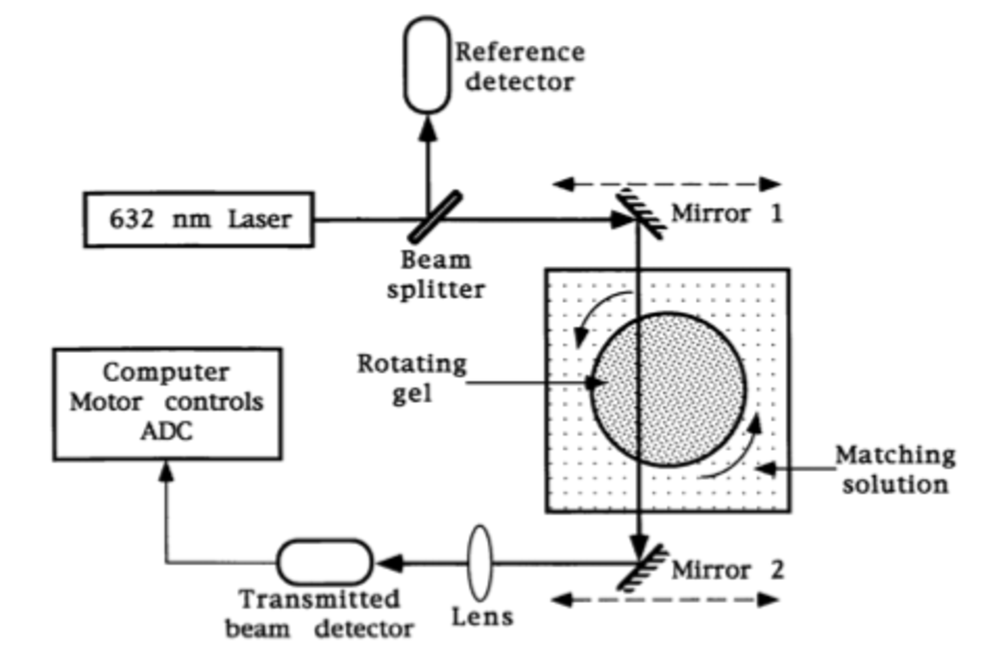
\includegraphics[scale=0.6]{Gore_setup.pdf}
\caption{A first generation,  Laser Scanning OptCT system developed by Gore. The sample is rotated and projections recorded at a number of angles. The  mirrors scan the laser beam across the sample but movement in the vertical direction is by manual adjustment only (figure from \cite{Gore:1999tg}). }
\label{fig:gore_setup}
\end{figure}


Laser scanning systems include a  beam splitter before the sample to create a reference beam. Dividing projections by the reference intensity  corrects for laser beam intensity fluctuations. \cite{Gore:1999tg}

Refraction and reflection at container walls are significant concerns for all configurations of dosimetry with OptCT. Generally, laser beams are incident on the gel container at a small angle, such as $5^{\circ}$, to avoid large reflection at the interface. In addition, the gel container is usually placed in a tank containing `matching fluid' with a refractive index close to that of the gel. This prevents significant refraction as the light passes into the gel. Doran found through ray tracing simulations that the refractive index of the walls of the matching tank and  gel container are not important compared to the gel and matching fluid. The optimum difference in refractive index between these two was calculated to be 0.0025 and not zero as originally thought.\cite{Doran:2001ee}

To maximise the dynamic range of the system, food dye is commonly added to the matching fluid so both the refractive index and optical density of the matching fluid and gel are very similar.\cite{Krstajic:2006kna} 




\subsection{Pixelated detector based systems}

In 1997 the first charge coupled device (CCD) camera based OptCT system was published by Tarte \textit{et al.} which employed an incoherent white light source and CCD camera detection. \cite{Tarte:2007} The advantage  of a pixelated detector based system  is that an entire 2-D projection can be imaged at once, potentially increasing the scanning speed by several  orders of magnitude depending on the data through-put rate. Tarte's system used a divergent light source and diffusing screen to measure optical density in a thin gel section (see Figure~\ref{fig:tarte_ccd_setup}). 
%For a very thin sample this adequate however, more sophisticated optics are required for bigger samples. \textbf{Does tarte reconstruct at all?}

\begin{figure}[H]
\centering
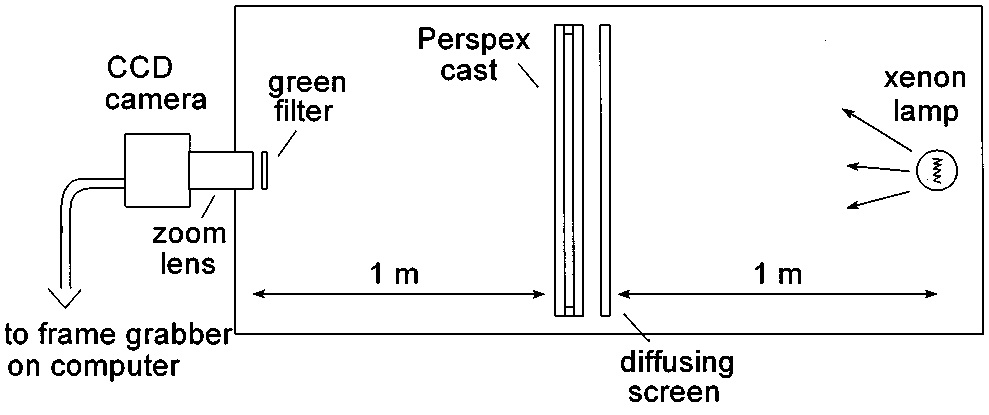
\includegraphics[scale=0.4]{Tarte_1997_ccdsetup.jpg}
\caption{Diagram of the first CCD-based  OptCT system, developed by Tarte \textit{et al.} It uses  divergent illumination from a white light source and CCD camera detection to record an entire 2D projection at once   (figure from \cite{Tarte:2007}). }
\label{fig:tarte_ccd_setup}
\end{figure}


The accuracy of Tarte's system  was checked by comparison with the standard measure of dosimetry, the parallel plate ionisation chamber. It was found to be on average within 3\% of the value from the ionisation chamber. \cite{Tarte:2007} A comparison between Tarte's laser scanning and CCD set-ups found that they had similar spatial resolutions. The CCD method had improved speed of acquistion but suffered from consistently worse SNR as a photodiode detector can collect many more photons per `pixel' than a CCD camera. \cite{Tarte:2007}

%The laser system 'pixel' is defined by the region illuminated by the laser spot while the photodiode has a much larger area than the spot, so it collects even photons which have diverged from a straight line. 

Advances in technology have meant that  high quality detectors are much more affordable. A cheaper alternative to very high quality CCD cameras is the CMOS (Complementary Metal-Oxide-Semiconductor) detector which has the potential for higher resolution and dynamic range. \cite{Doran:2008kh} Using a higher quality detector would improve many OptCT systems  in terms of scanning speed and reduced artefacts. \cite{Tarte:2007, Doran:2001ee}


\paragraph{Parallel beam configuration:} One method to reconstruct 3-D images with a CCD or CMOS detector is to create a broad parallel beam. This allows the use of parallel reconstruction algorithms, very similar to those used for x-ray CT. Each 2-D projection image recorded corresponds to one row for every slice in the 3-D reconstruction sinogram. \cite{Doran:2008kh}
Telecentric optics, in which the chief rays are parallel to the optical axis, are key in the design of this configuration. \cite{Walls:2005ja} Telecentric optics can be achieved either through a careful arrangement  of  a large converging lens before the sample and standard camera lens  \cite{Doran:2001ee} (see Figure~\ref{fig:doran_ccd_setup}) or through an expensive telecentric lens \cite{Sakhalkar:2008exa}. The process of forming a parallel beam results in non-uniformities in the lightfield. This is compensated for by subtracting a `correction' or `open lightfield', image which is a projection taken with no sample in the tank. \cite{Doran:2001ee}


\begin{figure}[H]
\centering
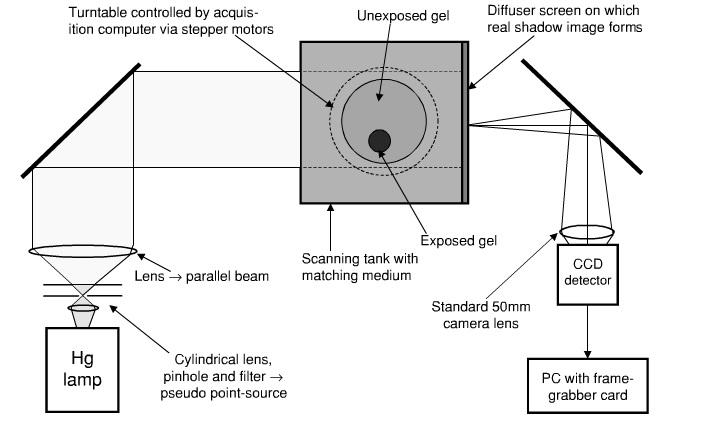
\includegraphics[scale=0.6]{Doran_2001_ccdsetup.jpg}
\caption{Diagram of a parallel beam  OptCT system, developed by Doran \textit{et al.} Telecentric optics create a parallel beam  (figure from \cite{Doran:2001ee}). }
\label{fig:doran_ccd_setup}
\end{figure}



Initial systems  suffered from `graininess' due to the unstable gain of cheap CCD cameras and granularity of the diffusing screen. \cite{Doran:2001ee}   Doran \textit{et al.} proposed some methods of correcting these problems. Oscillating the diffuser screen at high frequency 
``\,`smears' out the granularity'' while randomly horizontally displacing the CCD camera by a few pixels  between acquisitions can reduce the effect of `bad'  pixels.
 \cite{Doran:2001ee}
 The parallel configuration appears to be more susceptible to schlieren artefacts caused by refractive index inhomogeneities in the sample. \cite{Krstajic:2007hk}






\paragraph{Cone beam configuration:}
Wolodzko \textit{et al.} published the first cone beam OptCT system with CCD detection for gel dosimetry.\cite{Wolodzko:1999} One advantage of this configuration is the optics for producing a cone beam are much simpler than those for producing accurate parallel beams. \cite{Doran:2008kh} However, the reconstruction is computationally more complex. \cite{hsieh2003computed} A commercial cone-beam system, Vista\texttrademark by Modus Medical Devices Inc. (London, ON, Canada),  is available and reviewed recently by Olding \textit{et al.} \cite{Olding:2011eta}


\begin{figure}[H]
\centering
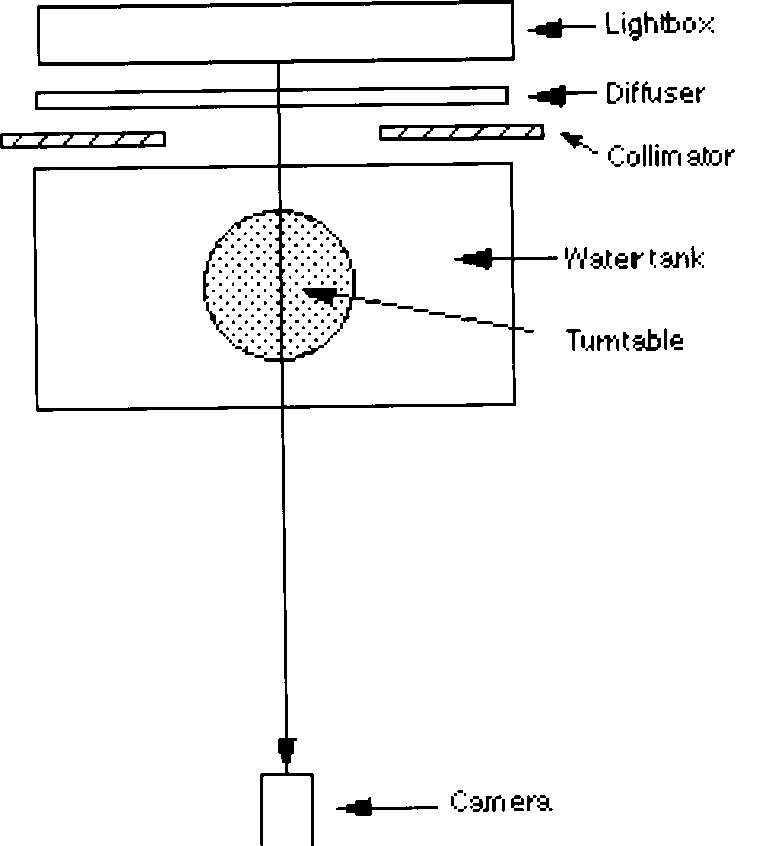
\includegraphics[scale=0.3]{Wolodzko_1999_conesetup.jpg}
\caption{Cone-beam CCD configuration (figure from \cite{Wolodzko:1999}).}
\end{figure}

When pixelated detectors are used, there appears to be more literature based on the parallel beam configuration than cone-beam. Although there has not been experimental comparison of the two Doran suggests that while cone-beam is usually somewhat cheaper due to simplified optics, modern parallel-beam systems have better scatter-rejection and may have fewer stray light problems. \cite{Doran:2008kh, Olding:2011eta, Thomas:2011eja}



 

 




%Refraction and reflection at container walls are significant concerns for all configuration of dosimetry with OptCT. These problems have been investigated with Mie theory modelling of light paths. Doran found through ray tracing simulations that the refractive index of the walls of the matching tank and  gel container are not important compared to the gel and matching fluid. The optimum difference in refractive index between these two was calculated to be 0.0025 and not zero as originally thought.\cite{Doran:2001ee} Another counter intuitive finding was that the ideal gel container wall thickness is not the thinnest possible but some median thickness which 

%Problems with vial walls misrepresentation due to refractive index mismatch. \cite{Doran:2001ee}

%Illumination is chosen based on the configuration used and the wavelength range which is optimum for dose measurement.  
%Stray light minimisation is very important in OptCT. Dark room, shield the illumination source. Interference filters. REF 
 

%Repeatability of experiments, have locking method for samples. REF
%Centre of rotation recovery, mostly post-processing. In theory section. 			

%\textit{The first is laser based and has several design considerations including minimisation of interference effects and stray light; scatter from optical components and the radiochromic gels themselves, reflection; dynamic range; wavelength selection; wall corrections plasma discharge from lasers; temperature changes; and the characterisation of detectors.A general disadvantage of scanners based on pixelated detectors together with a wide beam is the possible introduction of artefacts by refractive index inhomogeneities (schlieren). } from \cite{Doran:2008kh}







\newpage
\section{Optical Projection Tomography}

%Start with Sharpe's 2002 paper. What was his area? What adjustments did he make to the set-up for imaging organic tissue. What resolution, FOV possible. \cite{Sharpe:2002jp}

%Optical clearing required for imaging scattering material. Refer to section \ref{sec:clearing}

%Oldham also developing in this area. 


\section{Fluorescent OPT}
%Oldham has dual set-up. However, it was not originally quantitative. Just pretty pictures. Steps by various groups to get quantitative information out of emission. What is the change to the set-up?

%Imperial group investigating Opt combined with FRET and FLIM. Define these and some uses for the combined modality. Again, what physical/software changes needed for this imaging.
%\cite{McGinty:2008ix}

%Lorbeer - SLOT

\section{Optical Clearing}
\label{sec:clearing}

%Need for refractive index matching to ensure parallel beam assumption is true enough that we can emloy traditional reconstrion techniques. 

\section{Optical Staining}

\section{Recent Research}



\bibliography{bibliography2}

\end{document}